\section{Simulation}
\label{sec:av_simulation}

Once all the properties and modules are defined, the next step is to simulate the behavior of the autonomous vehicle in a controlled environment. The simulation provides a way to observe how the vehicle interacts with its surroundings, makes decisions, and executes actions based on the defined modules and properties. The enforcers are built in C using the easyRTE tool, while the simulation is run in Python as the models are developed in Python. The C code is execute through Python system calls. Figure \ref{fig:policy_implementation} shows the execution flow. At each time step, the enforcer checks the output of the module and corrects it if it violates the safety property. The corrected output is then passed to the controller, which in turn sends the corrected output to the car controls. The corrected output is then used to update the car's position and velocity.


\begin{figure}[htbp]
    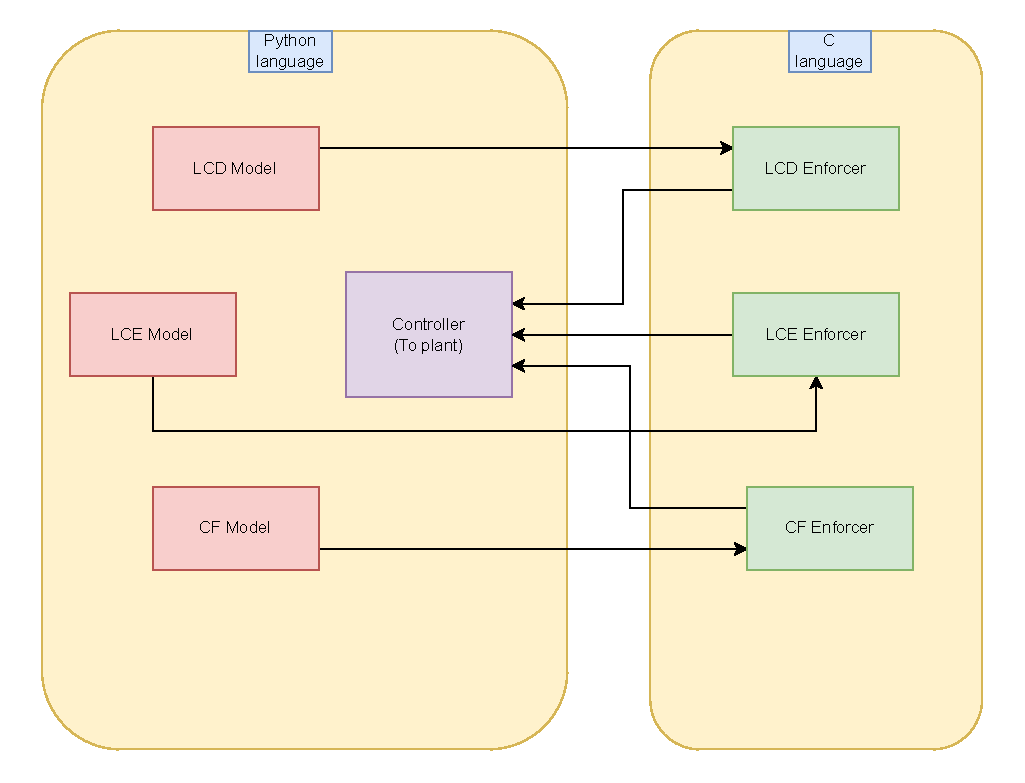
\includegraphics[width = \linewidth]{sections/av/fig/policy_implementation-2.pdf}
    \caption{Policy Implementation}
    \label{fig:policy_implementation}
\end{figure}


\begin{algorithm}[htbp]
    \caption{Autonomous Vehicle Simulation and Lane Change Model}
    \begin{algorithmic}[1]
    \State \textbf{Input:} Simulation duration $\text{sim\_duration\_sec}$, time step $\text{dt}$, number of lanes $\text{num\_lanes}$, list of cars $\mathcal{C}$, models for lane change and IDM.
    \State \textbf{Output:} History of car positions and velocities over time.
    
    \State \textbf{Step 1: Initialization}
    \State Initialize the IDM model and lane change model.
    \State Initialize controller for lane change execution.
    \State Initialize the cars with their positions, velocities, and lane assignments.
    \State Load pre-trained models for left, right, and center lane behaviors.
    
    \State \textbf{Step 2: Simulation Loop}
    \For{each time step $step$ in the range $\text{num\_steps}$}
        \State $current\_time \gets step \times dt$
        
        \State \textbf{Step 2.1: Data Collection and Processing}
        \State Collect data for left, right, and center lanes using the function $\text{get\_data}(\mathcal{C})$.
        \State Extract gap and lateral velocity information for ego car.
        
        \State \textbf{Step 2.2: Lane Change Decision}
        \State Compute lane change decision and prediction ($P$, $N$) with the collected data and pre-trained models.
        \State Pass data to enforcer and pass corrected (if needed) data to controller.
        \State Use the controller to process the inputs and determine lateral velocity setpoint.

        \State \textbf{Step 2.3: Lane Change Decision}
        \State Compute the car following behavior using the IDM model.
        \State Pass data to enforcer and pass corrected (if needed) data to controller.
        
        \State \textbf{Step 2.4: Lane Change Execution}
        \State Run lane change execution.
        \State Pass data to enforcer and pass corrected (if needed) data to controller.
        
        \State \textbf{Step 2.5: Update Vehicle Dynamics}
        \State Update ego car's lateral velocity and acceleration based on lane change and gap.
        \State Update longitudinal motion of all cars.
        \State Update lateral motion of cars.
        
        \State \textbf{Step 2.6: Lane Change Finalization}
        \If{car finishes lane change}
            \State Finalize the lane change and update the lane index and positions for the affected cars.
        \EndIf
        
        \State \textbf{Step 2.7: Store History}
        \State Append the current positions and velocities of each car to the history dictionary.
    \EndFor
    
    \State \textbf{Step 3: Return Results}
    \State Return the simulation history of all cars, including longitudinal and lateral positions, velocities.
    \end{algorithmic}
\end{algorithm}


\subsection{Simulation Algorithm}

To elaborate, the simulation operates in a synchronous, tick-based manner, where at each time step, or "tick," the entire system is updated simultaneously. Each tick represents a discrete time interval, and at every tick, the state of all vehicles in the simulation is updated at the same time. The current time is incremented by the time step $\text{dt}$, which is a constant value that determines the resolution of the simulation. This means that all vehicles are updated in parallel, and no vehicle progresses ahead or behind others in the simulation timeline.

At the start of each tick, data for every vehicle, such as its position, velocity, and other relevant parameters, is collected. This data is then used by the models, such as the lane change and Intelligent Driver Model (IDM), to compute the necessary actions for the current tick. These actions include deciding whether to change lanes, adjusting velocities, and updating positions. Importantly, all vehicles make these decisions simultaneously, based on their current states and the states of other vehicles in the environment.


Once a lane change decision is made, if applicable, the vehicle's lateral velocity and position are adjusted to execute the change. This happens for all vehicles that decide to change lanes during the current tick. Afterward, the vehicle dynamics are updated, meaning that the position of each vehicle is recalculated based on its velocity, considering any car-following behavior or lane changes that might have occurred. This synchronized update ensures that all vehicles' positions are accurate and that the dynamics of the system evolve coherently.

The simulation runs for a predefined number of ticks, which corresponds to the total simulation time. Each tick updates the vehicles' state, and this process continues until the end of the simulation. The synchronization of all updates at each tick ensures that interactions between vehicles, such as car-following and lane changing, are consistently executed in series.



The time step $\text{dt}$ is a key parameter in determining how frequently the system is updated. Smaller values of $\text{dt}$ lead to a finer resolution and more frequent updates, resulting in a more detailed simulation but at the cost of higher computational load. On the other hand, larger values of $\text{dt}$ reduce the computational cost but may introduce less accuracy in the modeling of vehicle behavior. Therefore, the choice of $\text{dt}$ needs to strike a balance between accuracy and efficiency, depending on the needs of the simulation. We choose $\text{dt} = 0.04$ seconds for our simulation, as the HighD dataset, which was used to obtain the LCD module data, has a time resolution of 0.04 seconds.



\subsection{Simulation set-up}

The simulation considers a three-lane roadway and operates with a time step ($\Delta t$) of 0.1 seconds as we believe this should be fast enough to make accurate decisions. We consider eight simulation durations, with the simulation duration varying linearly between 30 seconds and 480 seconds. The vehicle setup includes an ego vehicle positioned in the centre lane and six other vehicles distributed across adjacent lanes. The ego vehicle starts at the origin with an initial velocity of 20 m/s (desired velocity of 30 m/s) and occupies the centre lane. Surrounding vehicles are initialized with randomized positions and velocities to simulate a realistic driving environment. 

These vehicles are distributed across all three lanes, including vehicles in the same lane as the ego car and those in opposing and adjacent lanes. The randomized initial positions range from 2 to 100 meters from the ego car, while their velocities range from 5 to 30 m/s. Each vehicle is governed by an Intelligent Driver Model (IDM) for longitudinal control and a lane change model for lateral manoeuvres.

The execution of all the modules takes place in series every time instant. Each time instant, the car takes in the data from the car sensors and executes the LCD module and its enforcer, the LCE module and its enforcer and the CF module and its enforcer in series. Then, the results are passed to the controller to pass to the car, and the modules for the car to update its state begin the next step.The simulation is run in Python, but the enforcers are developed in C using the easyRTE tool.

To explore multiple scenarios, combinations of initial conditions and simulation durations are created using a Cartesian product of random seeds and duration intervals. We use ten randomised repetitions of the simulation durations, 80 simulations in total. The eight simulations with different simulation durations are parallelized using Python's multiprocessing library, enabling efficient execution across multiple CPU cores. 

As it may take a long time to observe undesired behaviour, we inject faults in the simulation to observe the behaviour of the AV  and whether the enforcer takes corrective action or not in the presence of faults. We inject the following faults in the simulation:

\begin{itemize}
    \item \textbf{Fault 1:} The LCD module outputs a lane change decision to the controller even when $P_{LCD} = 0$ is not met. This is introduced by setting the LCD output to 1 when $P_{LCD} = 0$ at multiples of time step 83.
    \item \textbf{Fault 2:} The car following distance becomes lesser than 2 metres. This is done by setting the gap to 1.99 metres at multiples of time step 89.
    \item \textbf{Fault 3:} The LCE module takes longer than 5 seconds for a lane change. This is done by artificially setting the lane change execution time to 5.04 seconds at multiples of time step 97.
\end{itemize}





